% Copyright (C) 2020 - Michael Baudin

\documentclass{beamer}

%\setbeameroption{hide notes}
%\setbeameroption{show notes}
%\setbeameroption{show only notes}

% Copyright (C) 2012 - EDF R&D - Michael Baudin

% To highlight source code
\usepackage{listings}
\definecolor{darkgreen}{rgb}{0,0.5,0}
\definecolor{violet}{rgb}{0.5,0,1}

\usepackage{lmodern}% http://ctan.org/pkg/lm

\usetheme{Montpellier}
\setbeamertemplate{navigation symbols}{} % Remove navigation
\useoutertheme{infolines}

\usepackage[utf8]{inputenc}
\usepackage[T1]{fontenc}

\usepackage{graphicx}
\unitlength=1cm
\graphicspath{{./figures/}}

\usepackage{hyperref}
\hypersetup{colorlinks=true, linkcolor=blue, linktocpage, urlcolor=blue}

\def\bx{{\bf x}}
\def\RR{\mathbb{R}}

\newcommand{\pyvar}[1]{\texttt{#1}}

\def \ot {OpenTURNS}

\definecolor{codegreen}{rgb}{0,0.6,0}
\definecolor{codegray}{rgb}{0.5,0.5,0.5}
\definecolor{codepurple}{rgb}{0.58,0,0.82}
\definecolor{backcolour}{rgb}{0.95,0.95,0.92}
\lstdefinestyle{mystyle}{
  backgroundcolor=\color{backcolour},   commentstyle=\color{codegreen},
  keywordstyle=\color{magenta},
  numberstyle=\tiny\color{codegray},
  stringstyle=\color{codepurple},
  basicstyle=\ttfamily\tiny,
  breakatwhitespace=false,         
  breaklines=true,                 
  captionpos=b,                    
  keepspaces=true,                 
  numbers=left,                    
  numbersep=5pt,                  
  showspaces=false,                
  showstringspaces=false,
  showtabs=false,                  
  tabsize=1,
  numbers=none
}

\lstset{style=mystyle, language=python}


\title[PERSALYS]{PERSALYS, the graphical interface of OpenTURNS}

\author[PERSALYS Team]{
M. Baudin \inst{1} \and
T. Delage \inst{1} \and
A. Dumas \inst{2} \and
A. Dutfoy \inst{1} \and \\
G. Garcia \inst{2} \and
A. Geay \inst{1} \and
O. Mircescu \inst{1} \and
A. Ladier \inst{2} \and \\
J. Schueller \inst{2} \and
T. Yalamas \inst{2}
}

\institute[EDF-Phiméca]{
\inst{1} EDF R\&D. 6, quai Watier, 78401, Chatou Cedex - France, michael.baudin@edf.fr \and %
\inst{2} Phimeca Engineering. 18/20 boulevard de Reuilly, 75012 Paris - France, yalamas@phimeca.com
}

\date[]{19 June 2020, OpenTURNS User's day}

%%%%%%%%%%%%%%%%%%%%%%%%%%%%%%%%%%%%%%%%%%%%%%%%%%%%%%%%%%%%%%%%%%%%%%%%%%%%%

  \begin{document}

%%%%%%%%%%%%%%%%%%%%%%%%%%%%%%%%%%%%%%%%%%%%%%%%%%%%%%%%%%%%%%%%%%%%%%%%%%%%%

\begin{frame}
  \titlepage
  
  \begin{columns}
    \column{0.45\textwidth}
  \begin{center}

\includegraphics[height=0.15\textheight]{figures/edf.jpg}
\end{center}
    \column{0.1\textwidth}
	
    \column{0.45\textwidth}
  \begin{center}

\includegraphics[height=0.15\textheight]{figures/logo_phimeca.png}
\end{center}
  \end{columns}

\end{frame}

\note{
I would like to thank the organizers to inviting us to present our tools. 
}

%%%%%%%%%%%%%%%%%%%%%%%%%%%%%%%%%%%%%%%%%%%%%%%%%%%%%%%%%%%%%%%%%%%%%%%%%%%%%

\begin{frame}
\frametitle{Contents}
\tableofcontents
\end{frame}

%%%%%%%%%%%%%%%%%%%%%%%%%%%%%%%%%%%%%%%%%%%%%%%%%%%%%%%%%%%%%%%%%%%%%%%%%%%%%

\section{Overview}

\begin{frame}
\frametitle{Bring Uncertainty Methodology to Engineers}
\begin{itemize}
\item 5 years ago

\begin{itemize}
\item EDF R\&D wants to maximize the use of OpenTURNS\textregistered{} by its engineer/researcher (and improve an existing GUI) => develop a GUI to make more easy to use

\item Phimeca has already developed an "OpenTURNS GUI" (PhimecaSoft\textregistered{}) which satisfy some needs of EDF R\&D but not all.

\item EDF R\&D and Phimeca decide to start a specific partnership in order to develop a new GUI based on OpenTURNS\textregistered{} and "Salome Tools": Paraview, Yacs, ...
\end{itemize}

\item Persalys is available, on Salome website, in EDF Specific Salome version and commercialized by Phimeca
\end{itemize}
\end{frame}

%%%%%%%%%%%%%%%%%%%%%%%%%%%%%%%%%%%%%%%%%%%%%%%%%%%%%%%%%%%%%%%%%%%%%%%%%%%%%
\begin{frame}
\frametitle{Some expectations regarding the GUI}
\begin{itemize}
\item As easy to use as possible and, when it is possible, a GUI which can guide the user 

\item Possibility to use it inside Salome Platform to 
\begin{itemize}
\item Use supercomputing resources (e.g. Gaïa, 3 052 Tflops peak, 41 000 cores)
\item Connect to EDF numerical code users (Code\_Aster for example)
\end{itemize}

\item Take benefit from the advanced visualization capability from Paraview

\item Drive the GUI from a python script usable in an "expert" mode
\end{itemize}
\end{frame}

%%%%%%%%%%%%%%%%%%%%%%%%%%%%%%%%%%%%%%%%%%%%%%%%%%%%%%%%%%%%%%%%%%%%%%%%%%%%%

\begin{frame}
\frametitle{PERSALYS, the graphical user interface of \ot{}}
	
\begin{itemize}
\item Main goal : provide a graphical interface of 
\ot{} in the SALOME integration platform
\item Features
	\begin{itemize}
	\item Uncertainty quantification : definition of the 
	probabilistic model (including dependence), distribution fitting (including 
	copulas), physical model with vector input 
	and vector output or 1D Fields,
	central tendency, sensitivity analysis, probability estimate, 
	metamodeling (polynomial chaos, kriging), screening (Morris), 
	optimization, design of experiments
	\item Generic (not dedicated to a specific application)
	\item GUI language : English, French
	\end{itemize}

\item Partners : EDF, Phiméca
\item Licence : LGPL

\item Schedule : 
	\begin{itemize}
	\item Since summer 2016, one EDF release per year
	\item On the internet (free) : SALOME\_EDF in the "CONTRIBUTIONS" section 
	since 2018 on \url{https://www.salome-platform.org}
	
	\end{itemize}

\end{itemize}

\end{frame}

\note{
We created a new tool within SALOME, called PERSALYS. 
}



%%%%%%%%%%%%%%%%%%%%%%%%%%%%%%%%%%%%%%%%%%%%%%%%%%%%%%%%%%%%%%%%%%%%%%%%%%%%%

\section{PERSALYS v8: Calibration}


%%%%%%%%%%%%%%%%%%%%%%%%%%%%%%%%%%%%%%%%%%%%%%%%%%%%%%%%%%%%%%%%%%%%%%%%%%%%%

\begin{frame}
\frametitle{Calibration}

Given a physical model $H$, observed inputs $x$, 
observed outputs $y$ we can calibrate $\theta$ so that 
$$
y_i = H(x_i, \theta) + \epsilon
$$
where $\epsilon$ is a random variable.

Calibration outputs:
\begin{itemize}
\item the optimal value $\theta^\star$,
\item the distribution of $\theta^\star$,
\item the distribution of the residuals $r_i = y_i - H(x_i, \theta^\star)$.
\end{itemize}

This allows to get confidence intervals of $\theta^\star$.

\end{frame}

%%%%%%%%%%%%%%%%%%%%%%%%%%%%%%%%%%%%%%%%%%%%%%%%%%%%%%%%%%%%%%%%%%%%%%%%%%%%%

\begin{frame}
\frametitle{Calibration}

In PERSALYS, this requires:
\begin{itemize}
\item a physical model $H$, 
\item a data file containing the observed inputs and outputs.
\end{itemize}

\begin{center}
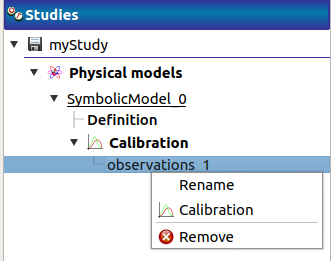
\includegraphics[width=0.4\textwidth]{figures/observations_contextMenu.png}
\end{center}

\end{frame}

%%%%%%%%%%%%%%%%%%%%%%%%%%%%%%%%%%%%%%%%%%%%%%%%%%%%%%%%%%%%%%%%%%%%%%%%%%%%%

\begin{frame}
\frametitle{Calibration}
	
\begin{center}
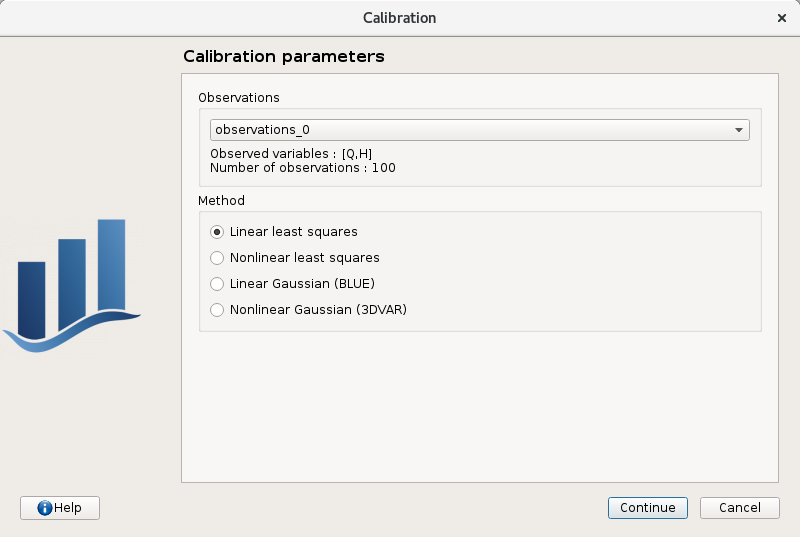
\includegraphics[width=0.7\textwidth]{figures/calibration_algorithms.png}
\end{center}

\end{frame}


%%%%%%%%%%%%%%%%%%%%%%%%%%%%%%%%%%%%%%%%%%%%%%%%%%%%%%%%%%%%%%%%%%%%%%%%%%%%%

\begin{frame}
\frametitle{Calibration}
	
\begin{center}
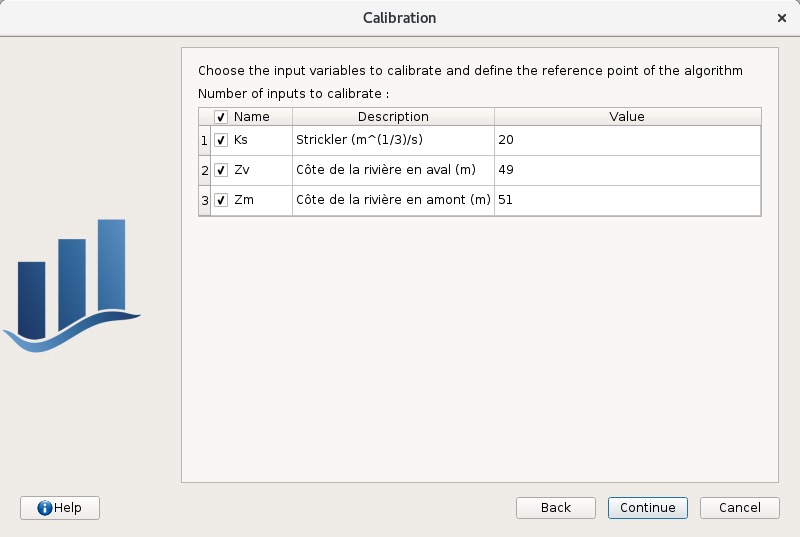
\includegraphics[width=0.9\textwidth]{figures/calibration-Parametres.png}
\end{center}

\end{frame}

%%%%%%%%%%%%%%%%%%%%%%%%%%%%%%%%%%%%%%%%%%%%%%%%%%%%%%%%%%%%%%%%%%%%%%%%%%%%%

\begin{frame}
\frametitle{Calibration}
	
\begin{center}
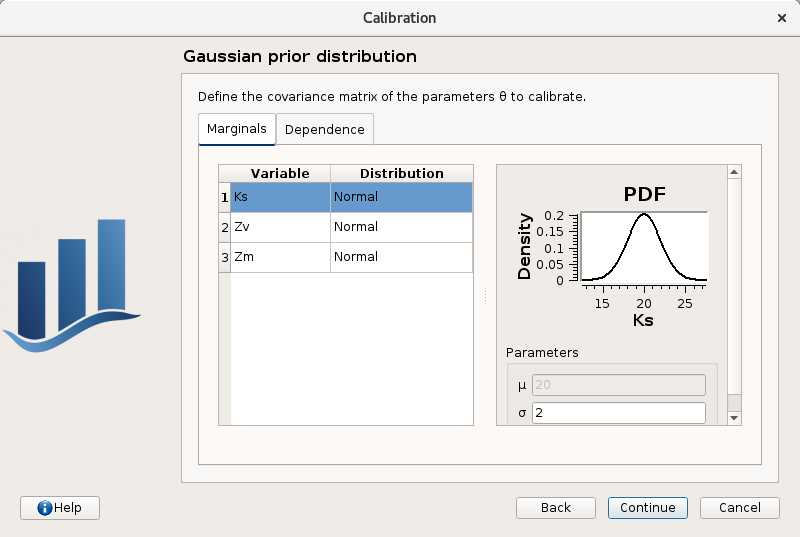
\includegraphics[width=0.9\textwidth]{figures/calibration-Gaussien-prior.png}
\end{center}

\end{frame}

%%%%%%%%%%%%%%%%%%%%%%%%%%%%%%%%%%%%%%%%%%%%%%%%%%%%%%%%%%%%%%%%%%%%%%%%%%%%%

\begin{frame}
\frametitle{Calibration}
	
\begin{center}
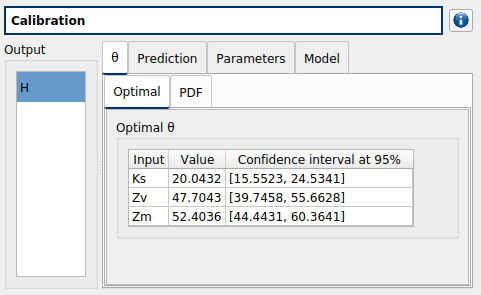
\includegraphics[width=0.7\textwidth]{figures/calibration-ks-zv-zm-optimal.png}
\end{center}

\end{frame}

%%%%%%%%%%%%%%%%%%%%%%%%%%%%%%%%%%%%%%%%%%%%%%%%%%%%%%%%%%%%%%%%%%%%%%%%%%%%%

\begin{frame}
\frametitle{Calibration}
	
\begin{center}
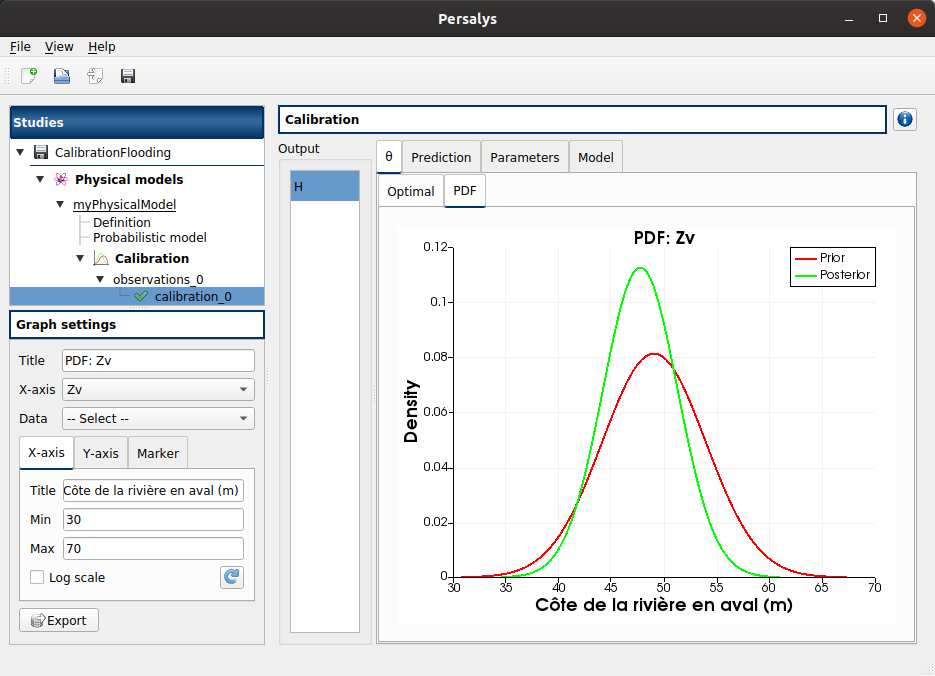
\includegraphics[width=0.9\textwidth]{figures/calibration-Zv-prior-posterior.png}
\end{center}

\end{frame}

%%%%%%%%%%%%%%%%%%%%%%%%%%%%%%%%%%%%%%%%%%%%%%%%%%%%%%%%%%%%%%%%%%%%%%%%%%%%%

\begin{frame}
\frametitle{Calibration}
	
\begin{center}
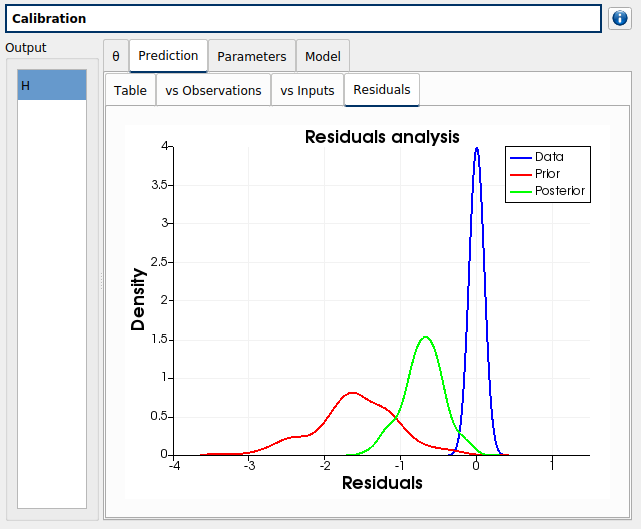
\includegraphics[width=0.7\textwidth]{figures/calibration-residual-analysis.png}
\end{center}

\end{frame}

\note{
Rouge : la distribution des résidus avant calage.
Vert : la distribution des résidus après calage.
Bleu : la distribution gaussienne des résidus. Gaussien (TODO : préciser)
}

%%%%%%%%%%%%%%%%%%%%%%%%%%%%%%%%%%%%%%%%%%%%%%%%%%%%%%%%%%%%%%%%%%%%%%%%%%%%%

\begin{frame}
\frametitle{Calibration}
	
\begin{center}
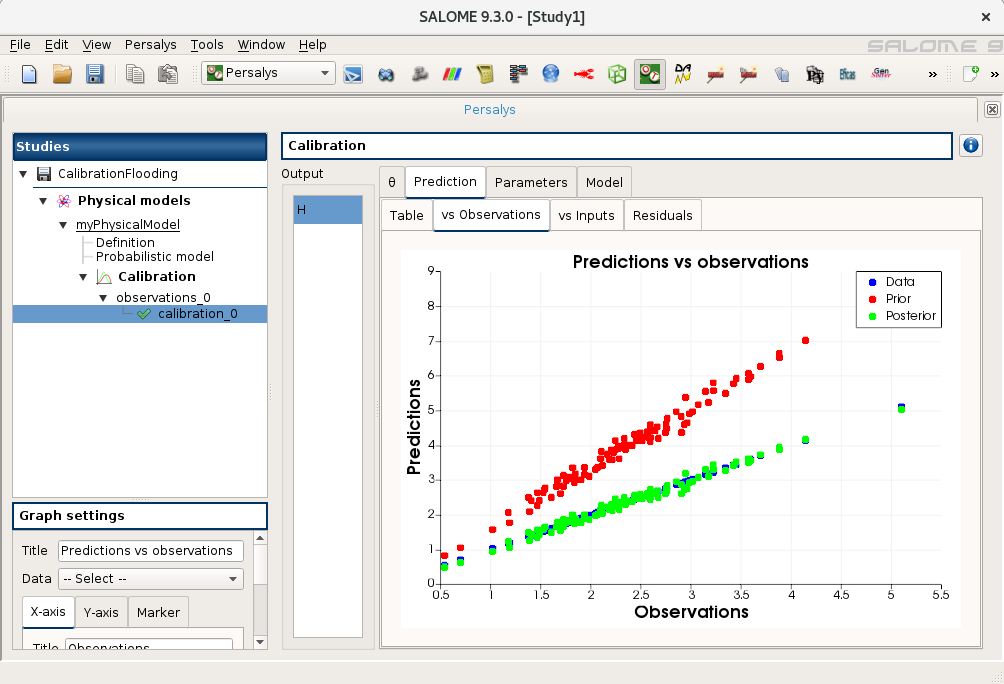
\includegraphics[width=0.9\textwidth]{figures/calibration-Resultat-3DVAR.png}
\end{center}

\end{frame}

%%%%%%%%%%%%%%%%%%%%%%%%%%%%%%%%%%%%%%%%%%%%%%%%%%%%%%%%%%%%%%%%%%%%%%%%%%%%%

\section{Coupling tools}

\begin{frame}
\frametitle{Coupling with external code}

A new physical coupling dialog was created:
\begin{itemize}
\item Execute any computer code from system e.g. with command line statement
\item Create a pipeline of commands
\item Exchange data with input and output files
\item Manage input and output cache to save simulations
\item Can be parallel : multithread or distributed (in SALOME)
\item Makes the tuning of input template file and the reading of output files easy
\end{itemize}

\end{frame}

%%%%%%%%%%%%%%%%%%%%%%%%%%%%%%%%%%%%%%%%%%%%%%%%%%%%%%%%%%%%%%%%%%%%%%%%%%%%%

\begin{frame}
\frametitle{Coupling with external code}

\begin{center}
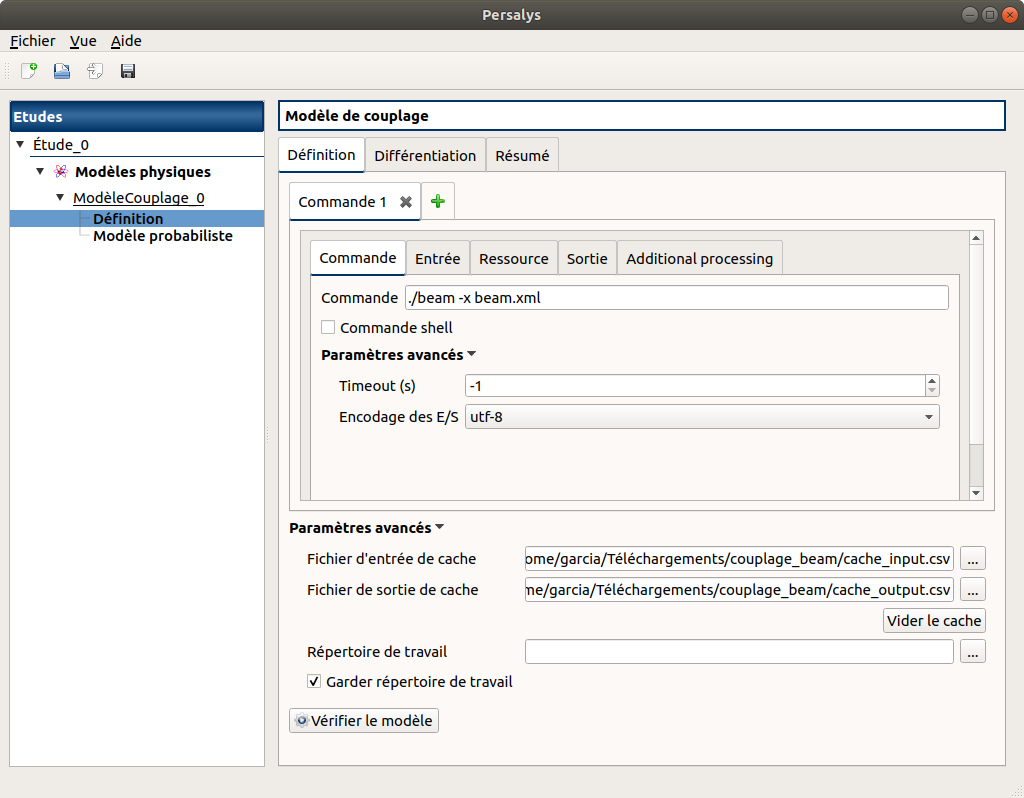
\includegraphics[width=0.7\textwidth]{figures/coupling-1-Commande.png}
\end{center}

\end{frame}

%%%%%%%%%%%%%%%%%%%%%%%%%%%%%%%%%%%%%%%%%%%%%%%%%%%%%%%%%%%%%%%%%%%%%%%%%%%%%

\begin{frame}
\frametitle{Coupling with external code}

A diff can be generated between the input template and the actual input file.

\begin{center}
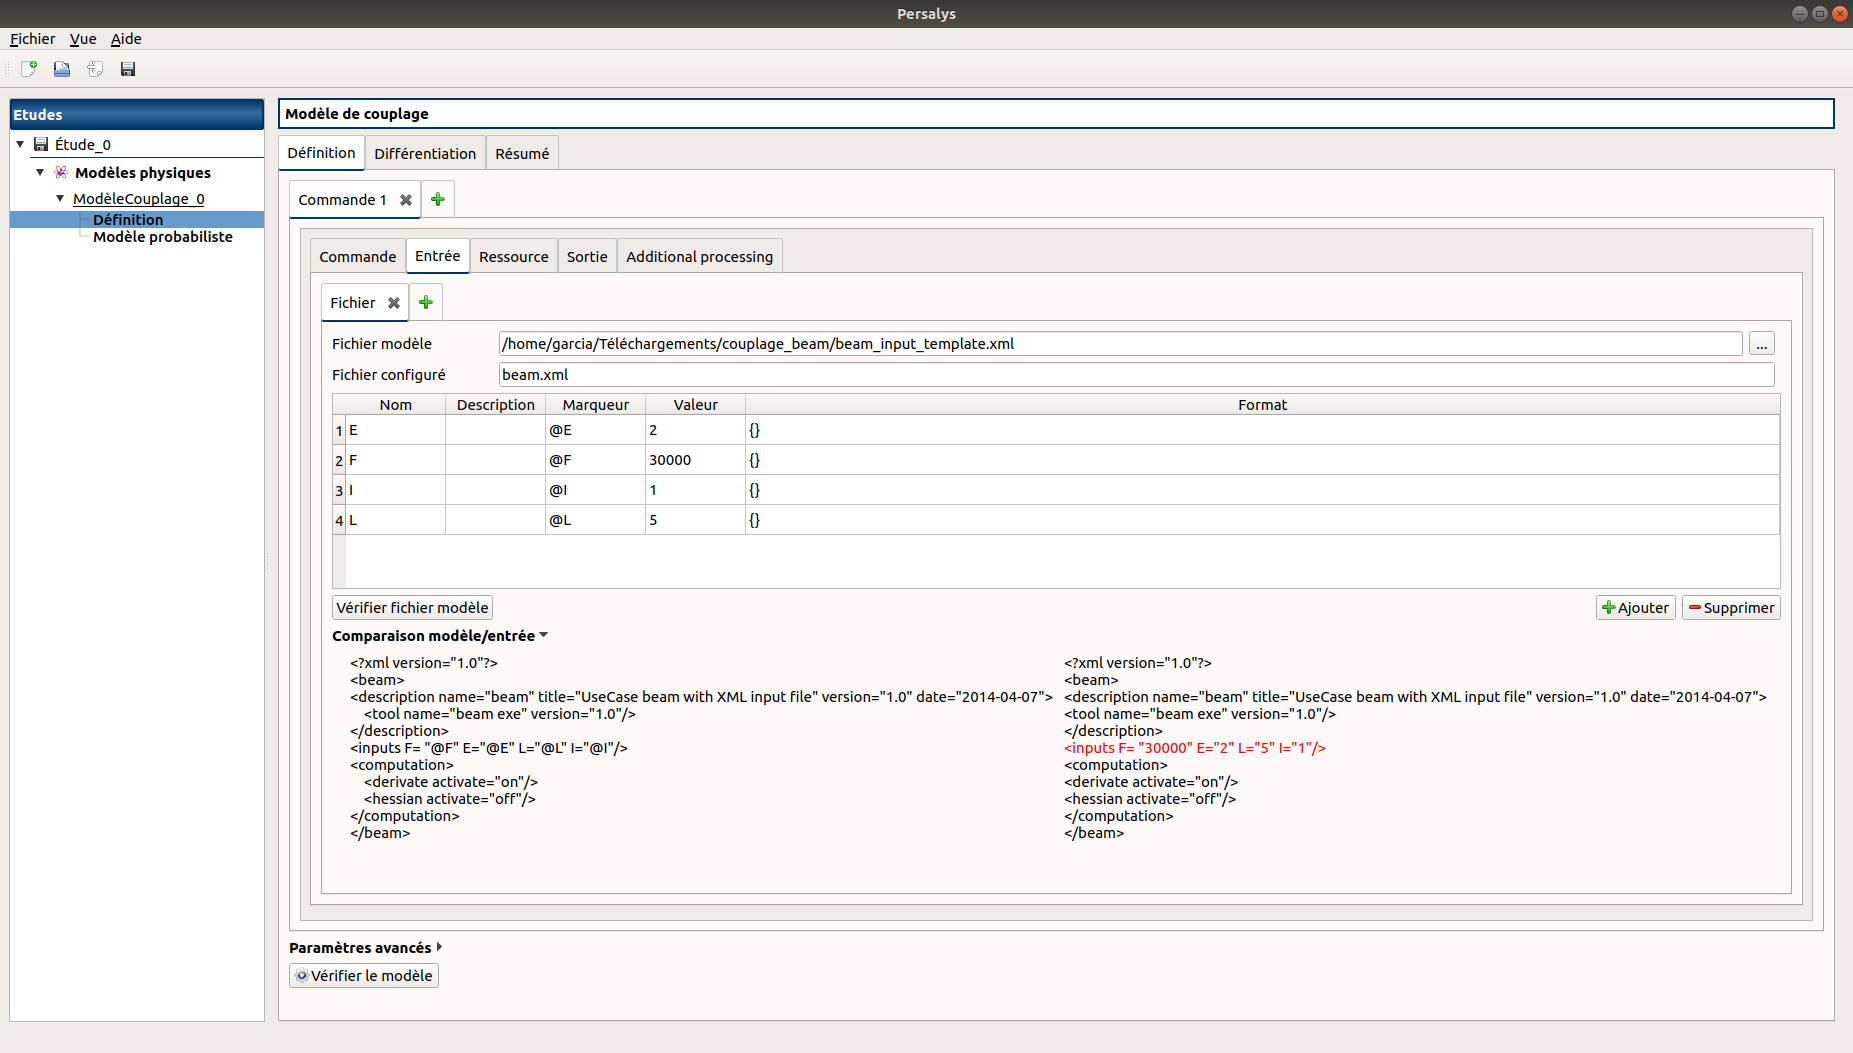
\includegraphics[width=0.9\textwidth]{figures/coupling-2-Entree.png}
\end{center}

\end{frame}

%%%%%%%%%%%%%%%%%%%%%%%%%%%%%%%%%%%%%%%%%%%%%%%%%%%%%%%%%%%%%%%%%%%%%%%%%%%%%

\begin{frame}
\frametitle{Coupling with external code}

Resources are files to copy to run the simulation : mesh, parameters, etc...

\begin{center}
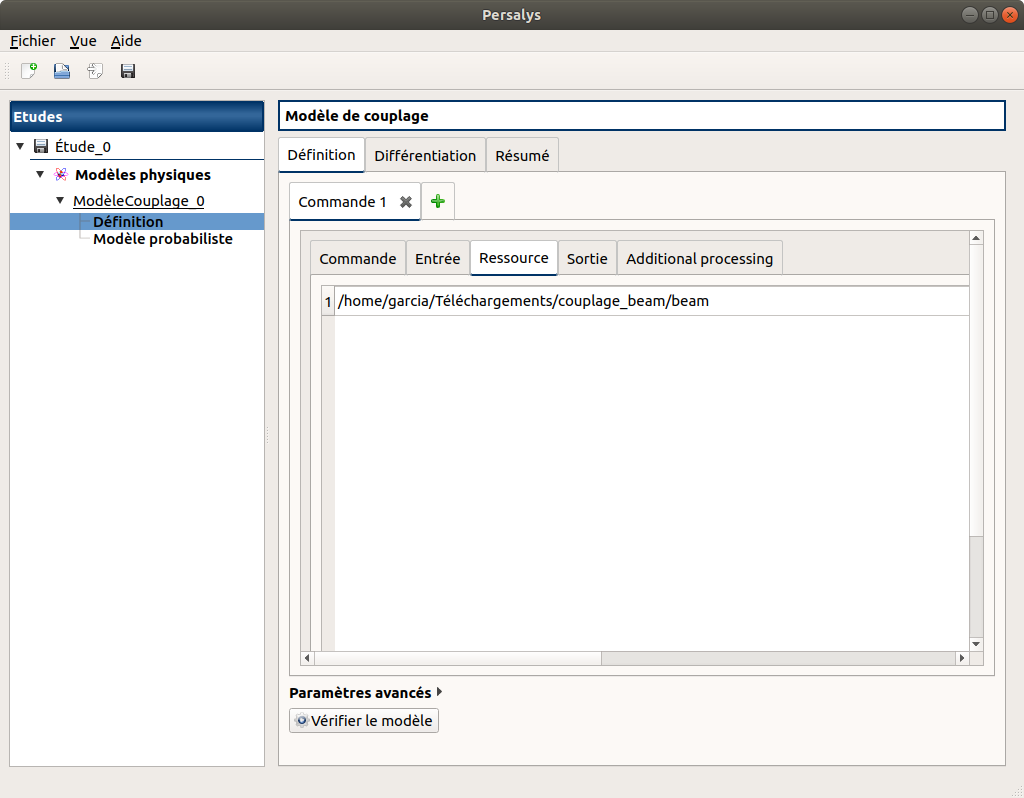
\includegraphics[width=0.8\textwidth]{figures/coupling-3-Ressource.png}
\end{center}

\end{frame}

%%%%%%%%%%%%%%%%%%%%%%%%%%%%%%%%%%%%%%%%%%%%%%%%%%%%%%%%%%%%%%%%%%%%%%%%%%%%%

\begin{frame}
\frametitle{Coupling with external code}

\begin{center}
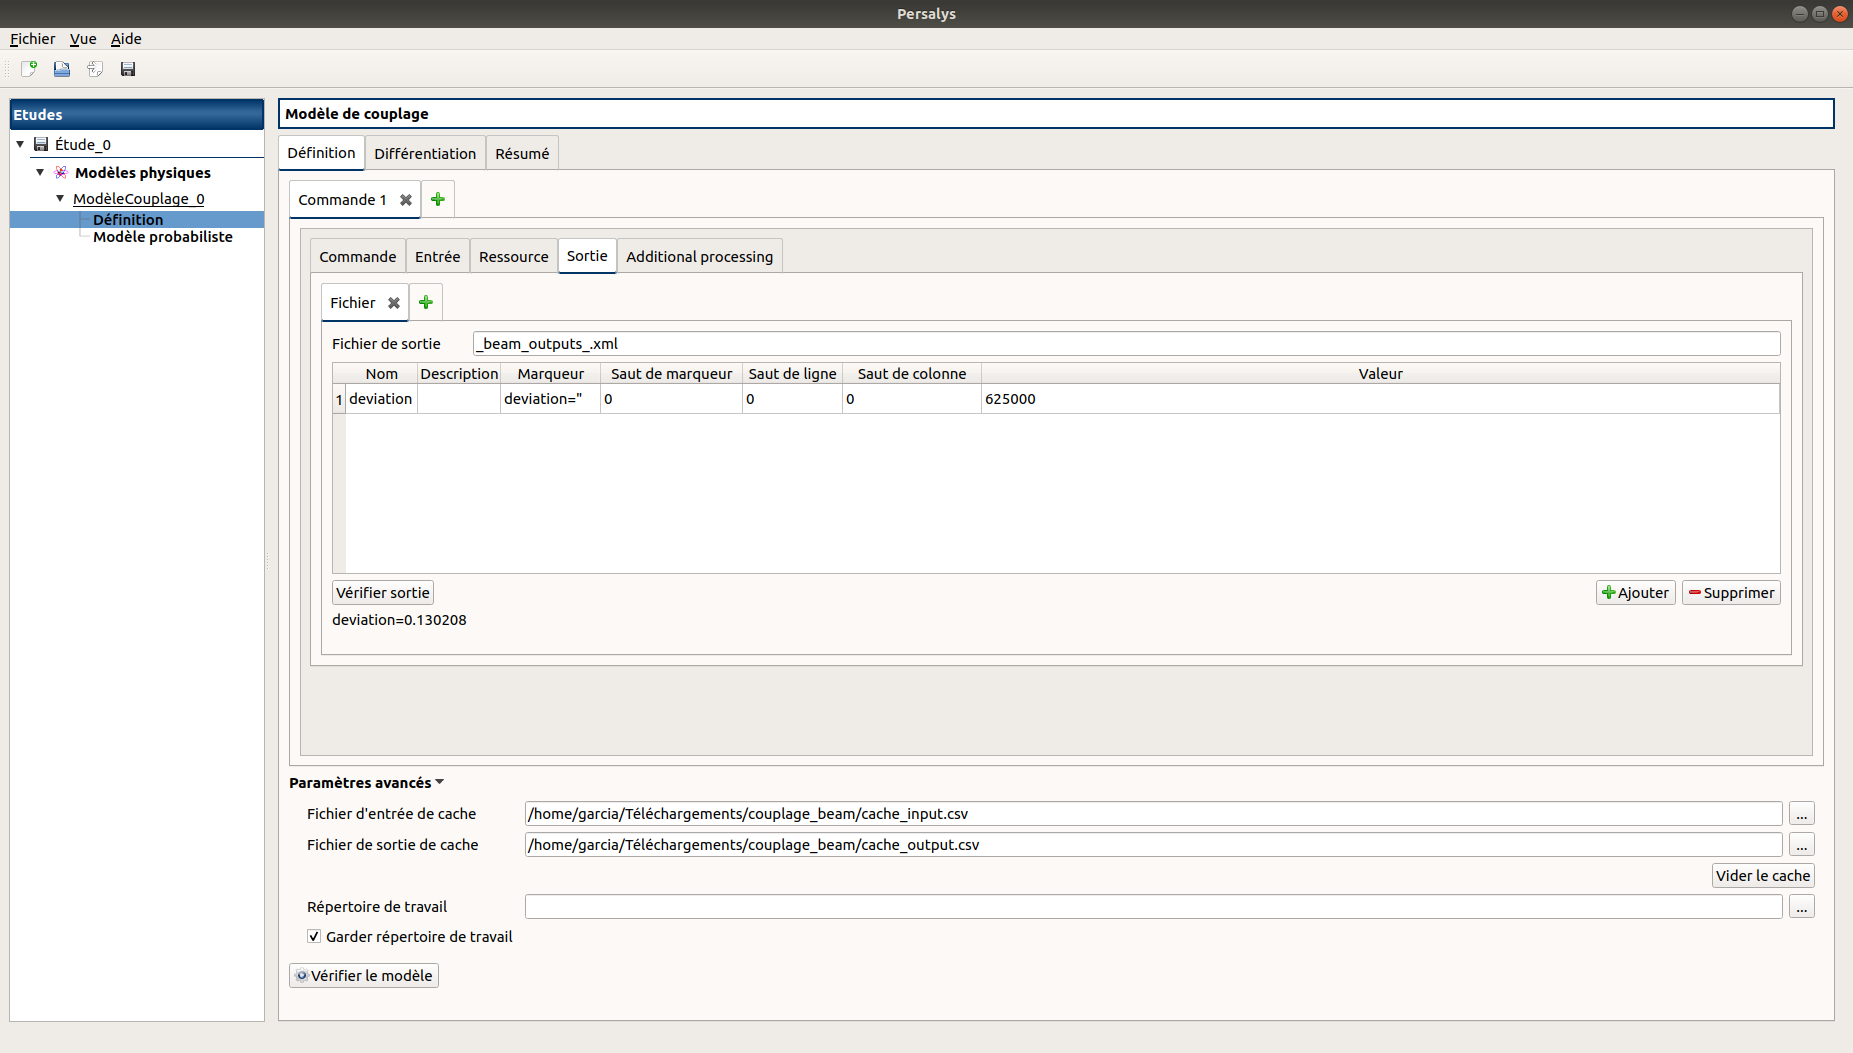
\includegraphics[width=1.0\textwidth]{figures/coupling-4-sortie.png}
\end{center}

\end{frame}

%%%%%%%%%%%%%%%%%%%%%%%%%%%%%%%%%%%%%%%%%%%%%%%%%%%%%%%%%%%%%%%%%%%%%%%%%%%%%

\begin{frame}
\frametitle{Coupling with external code}

On-disk cache management: one input point X is only evaluated once. 

\begin{center}
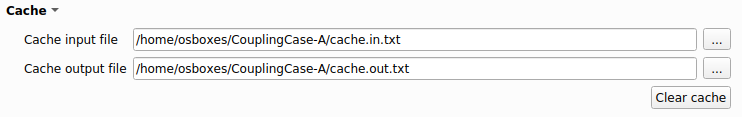
\includegraphics[width=0.8\textwidth]{figures/coupling-cache-focus.png}
\end{center}

\end{frame}

%%%%%%%%%%%%%%%%%%%%%%%%%%%%%%%%%%%%%%%%%%%%%%%%%%%%%%%%%%%%%%%%%%%%%%%%%%%%%

\section{Website}

\begin{frame}
\frametitle{Website}

\url{persalys.fr} : download (source, binaries), doc (videos tutorials), news
	
\begin{center}
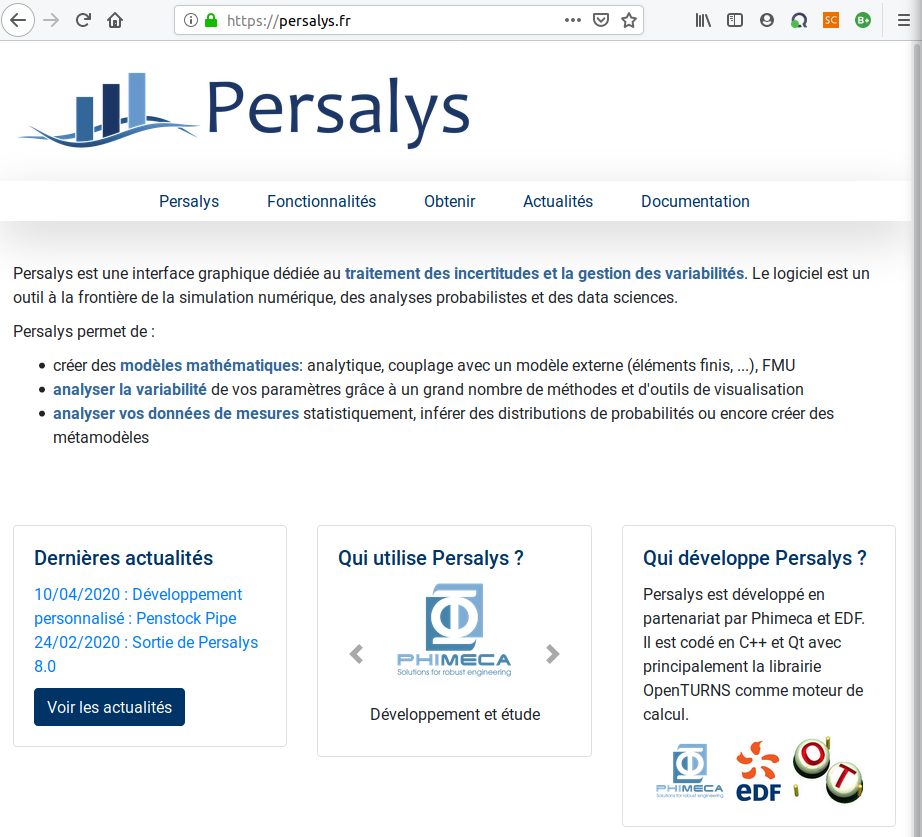
\includegraphics[width=0.6\textwidth]{figures/persalys-web.png}
\end{center}

\end{frame}

%%%%%%%%%%%%%%%%%%%%%%%%%%%%%%%%%%%%%%%%%%%%%%%%%%%%%%%%%%%%%%%%%%%%%%%%%%%%%

\section{What's next ?}

\begin{frame}
\frametitle{What's next ?}
  \begin{columns}
    \column{0.5\textwidth}

PERSALYS Roadmap : 
\begin{itemize}
\item 2D Fields, 3D Fields
\item In-Situ fields based on the MELISSA library (with INRIA): 
when we cannot store the whole sample in memory or on the hard drive, 
update the statistics (e.g. the mean, Sobol' indices) sequentially, 
with distributed computing. 
\item Linear regression.
\end{itemize}

    \column{0.5\textwidth}

\begin{center}
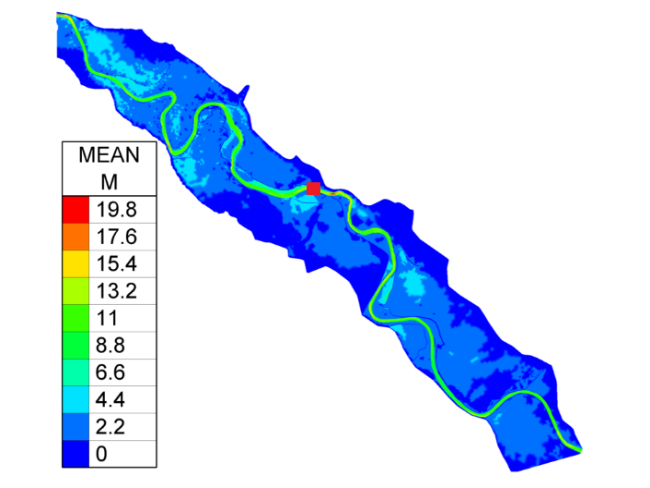
\includegraphics[height=0.5\textheight]{figures/image034.png}
\end{center}

	\end{columns}

\end{frame}

\note{
We are currently working on adding features to perform 
the calibration of a computer code (almost done). 

The next features we plan to add to PERSALYS are the management 
of 2D and 3D stochastic fields. 

We also work on the use of the MELISSA software which performs 
in-situ studies. 

This library allows to perform UQ studies in situations 
where we cannot store more than a couple of multidimensional fields 
in memory or on the hard drive. 
}

%%%%%%%%%%%%%%%%%%%%%%%%%%%%%%%%%%%%%%%%%%%%%%%%%%%%%%%%%%%%%%%%%%%%%%%%%%%%%

\begin{frame}
\frametitle{The end}

\begin{center}
Thanks !
\end{center}

\begin{center}
Questions ?
\end{center}

\end{frame}

\note{
Thank you for your attention. 

If you have any question, it would be a pleasure to answer them. 

If you want a live demo of PERSALYS, I can show you during the coffee break.
}

% %%%%%%%%%%%%%%%%%%%%%%%%%%%%%%%%%%%%%%%%%%%%%%%%%%%%%%%%%%%%%%%%%%%%%%%%%%%%%

%\section{PERSALYS, the graphical user interface}

\begin{frame}
\frametitle{SALOME}

  \begin{columns}
    \column{0.5\textwidth}
	
\begin{itemize}
\item Integration platform for pre and post processing, and 2D/3D numerical simulation 
\item Features : geometry, mesh, distributed computing
\item Visualization, data assimilation, uncertainty treatment
\item Partners : EDF, CEA, Open Cascade
\item Licence : LGPL
\item Linux, Windows
\item \url{www.salome-platform.org}
\end{itemize}

    \column{0.5\textwidth}

\begin{center}
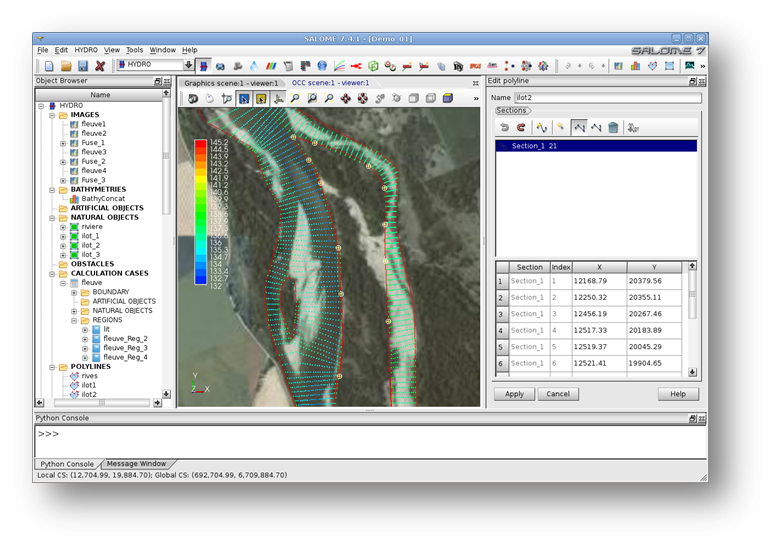
\includegraphics[width=0.95\textwidth]{figures/Salome-hydro-platform}
\end{center}

	\end{columns}
\end{frame}

\note{
Before presenting the graphical user interface, I would like to say some 
words about SALOME.
}

%%%%%%%%%%%%%%%%%%%%%%%%%%%%%%%%%%%%%%%%%%%%%%%%%%%%%%%%%%%%%%%%%%%%%%%%%%%%%

\begin{frame}
\frametitle{PERSALYS: 1D fields}
	
\begin{itemize}
\item Karhunen Loeve decomposition
\item Show modes, eigenvalues and projection coefficients
\end{itemize}

\begin{center}
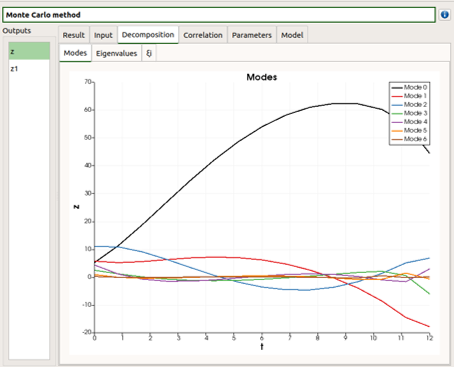
\includegraphics[width=0.45\textwidth]{figures/persalys-field-modes.png}
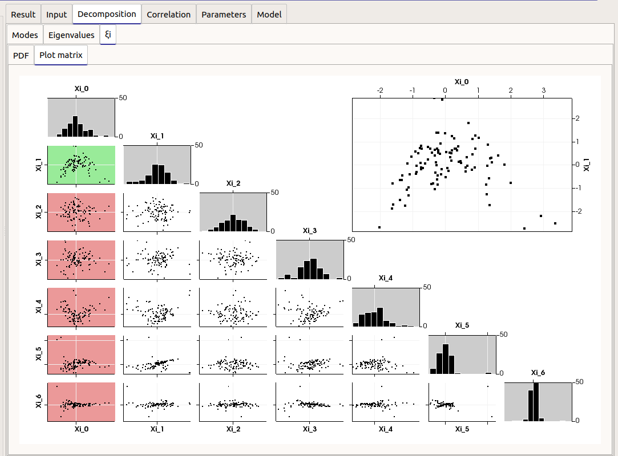
\includegraphics[width=0.45\textwidth]{figures/persalys-field-plotmatrix-extract.png}
\end{center}

\end{frame}
%%%%%%%%%%%%%%%%%%%%%%%%%%%%%%%%%%%%%%%%%%%%%%%%%%%%%%%%%%%%%%%%%%%%%%%%%%%%%
%\section{Extra slides}

\begin{frame}
\frametitle{Interactive uncertainty visualization with Paraview}

\begin{center}
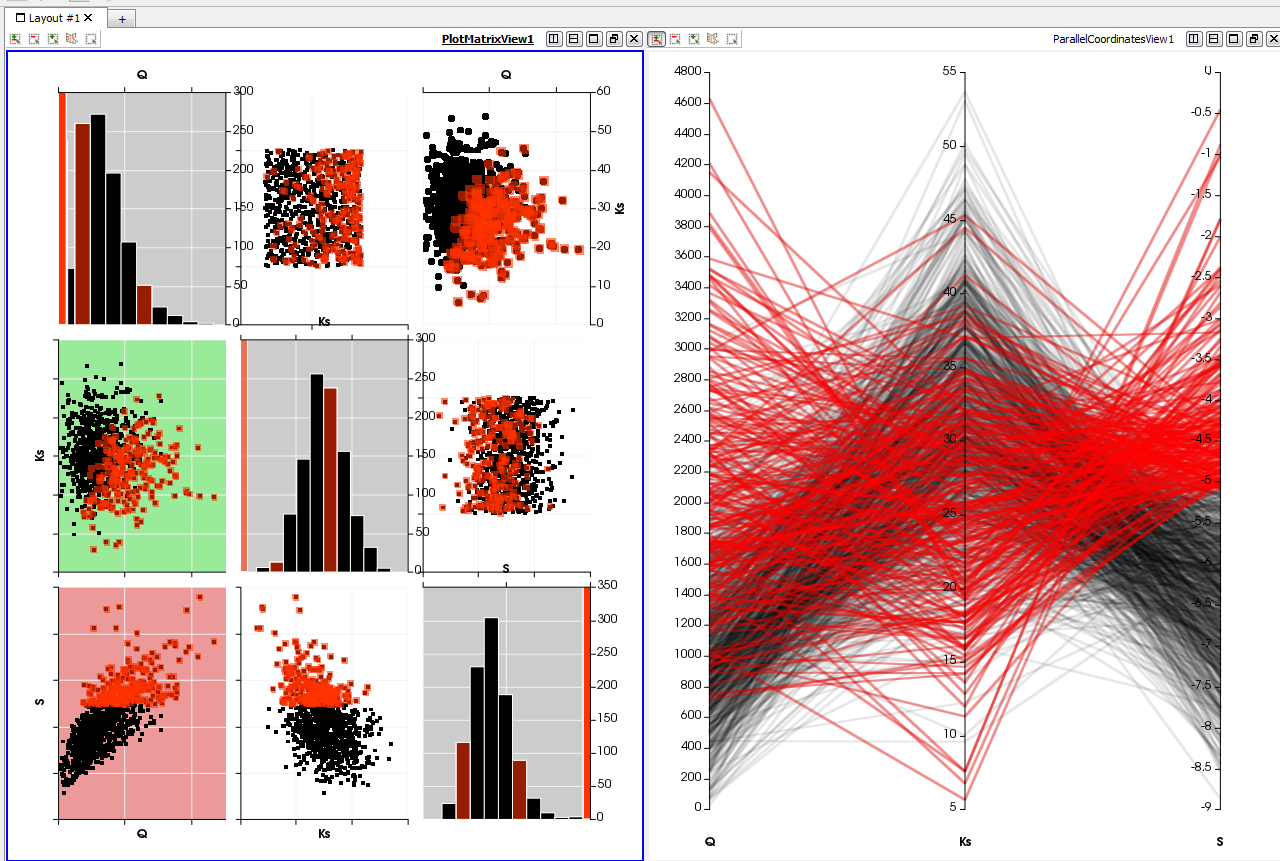
\includegraphics[width=0.9\textwidth]{figures/image032.png}
\end{center}

\end{frame}


%%%%%%%%%%%%%%%%%%%%%%%%%%%%%%%%%%%%%%%%%%%%%%%%%%%%%%%%%%%%%%%%%%%%%%%%%%%%%

\begin{frame}
\frametitle{1D fields}
	
\begin{itemize}
\item Probabilistic model
\item Uncertainty propagation with simple Monte-Carlo sampling
\end{itemize}

\begin{center}
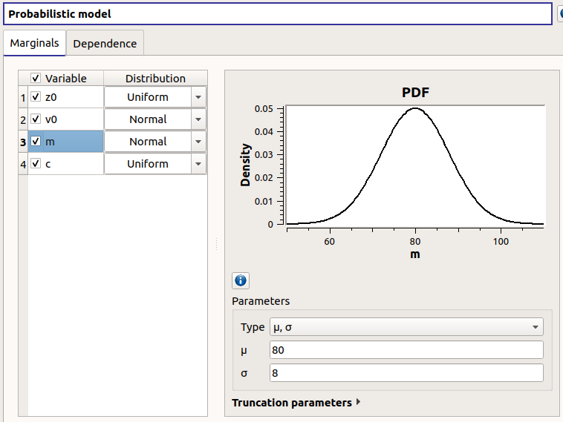
\includegraphics[width=0.45\textwidth]{figures/persalys-field-probabilistic-model.png}
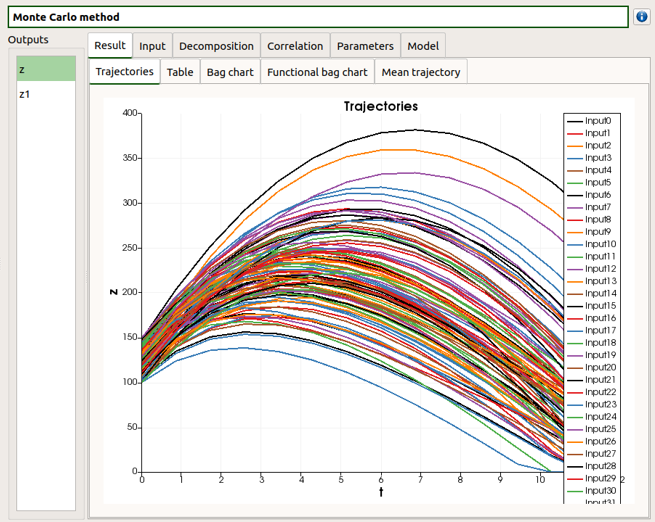
\includegraphics[width=0.45\textwidth]{figures/persalys-field-montecarlo-trajectories-extract.png}
\end{center}

\end{frame}

\note{
Then we can perform the central dispersion analysis of the model. 

On the left, we define the distribution of the input random vector. 

On the right, this is the result of the simulation: a sample made 
of 100 (one hundred) trajectories. 
}
%%%%%%%%%%%%%%%%%%%%%%%%%%%%%%%%%%%%%%%%%%%%%%%%%%%%%%%%%%%%%%%%%%%%%%%%%%%%%

\begin{frame}
\frametitle{1D fields}
	
\begin{itemize}
\item BagChart and Functional Bagchart (from Paraview) 
based on High Density Regions (Hyndman, 1996).
\item To do this, Paraview uses a principal component analysis  
decomposition. 
\item Linked and interactive selections in the views. 
\end{itemize}

\begin{center}
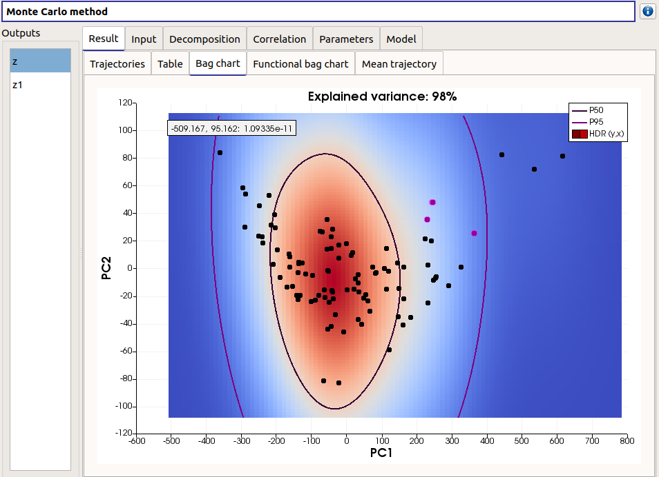
\includegraphics[width=0.45\textwidth]{figures/persalys-field-bagchart.png}
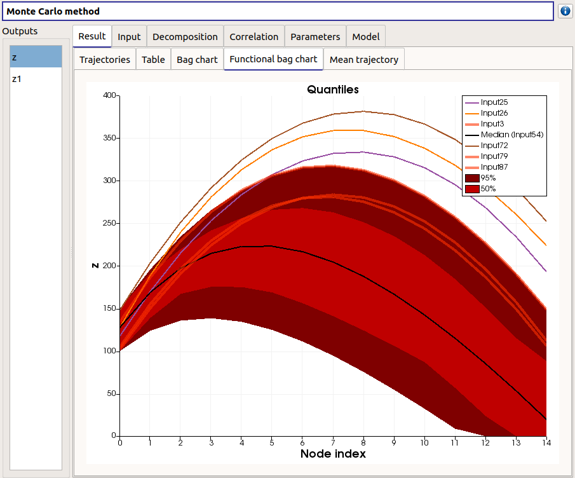
\includegraphics[width=0.45\textwidth]{figures/persalys-field-functional-bagchart.png}
\end{center}

\end{frame}

\note{
To analyze these trajectories requires more advanced tools than with 
classical multivariate samples, so that we can take into account for the 
time dependence. 

We use the BagChart and Functional Bagchart (from Paraview) tools, 
which uses the High Density Regions algorithm . 
}


\end{document}
